\section{Demonstrations: complete traces from source to question}
\label{sec:demos}

The tables in \cref{sec:n2,sec:n3} report counts. This section follows one record end to end
(source, verbatim span, claim and label, lens, inferred gap, hypothesis and generated question) and
one record kept to show a known defect. Two further traces, one from each GDPR run, are in
\cref{app:records}. Quoted fields are copied from the committed \code{gapmap.json} files; where we
shorten, we say so. \textbf{Every record below is a candidate.} No expert has read or answered any of
these questions.

\evobs{} The traces were chosen by the author after the maps were final. The rule, stated after the
fact, is: the top-ranked record of each map, plus PLC's second record as a failure example. They are
not a random sample, and the top-ranked records are among the richest in the maps.

\subsection{Trace 1: PLC, rival causes of an intermittent fault}

PLC's top-ranked record merges six lens records into one DIAG group.\footnote{\repo{research/n3/plc/gapmap.json},
\code{map[0]}, \code{gap_id} \code{g-59164a9db5bd}; also \repo{research/n3/plc/gapmap.md},
\enquote{\#1 [DIAG]}.} \Cref{tab:trace1} gives the record and \cref{fig:trace} draws it.

\begin{table}[tbp]
  \centering
  \small
  \caption{Trace 1: PLC, lens DIAG, gap \code{g-59164a9db5bd}, category HYP, closure \code{open}.}
  \label{tab:trace1}
  \begin{tabularx}{\linewidth}{@{}p{2.4cm}X@{}}
    \toprule
    Stage & Content \\
    \midrule
    Seed source & \url{liambee.me/general/troubleshooting-plc-systems-a-systematic-approach-to-finding-faults} \\
    Seed span (verbatim) & \enquote{Loose terminals cause many intermittent faults. A flashlight
      reveals problems in dark panels that you miss otherwise.} \\
    Seed claim / label & \code{c-d7bce12d16755797}, \code{literature_supported}, verdict
      \code{supports}. The extractor's assertion, which the lens reads: \enquote{Loose terminal
      connections are a common cause of intermittent PLC faults and should be checked during
      troubleshooting.} The anchor is this assertion cut at 80 characters. \\
    Lens \& target & DIAG: 7 independent sources discuss the topic; the lens found 5 rival causes
      (ground loops, aliasing, installation vs.\ software, VFD/contactor noise, pull-up/clock
      timing) \\
    Inferred gap & Of 34 verified sentences retrieved, the judge found none that fully states a
      discriminating sign for any of the 5 rival causes; it marked 5 claims as partial (e.g.,
      \enquote{Sentences 1 and 4 partially address the distinction but do not explicitly state an
      observable sign}). DIAG treats a partially signed rival as unsigned, so the group reads
      \code{open}. \\
    Hypothesis (inferred) & \enquote{\ldots{} practitioners are predicted to tell these rival causes
      of \enquote{Loose terminal connections are a common cause of intermittent PLC faults and} apart
      by signs; the closure judge found a sign for the following (test DIAG:c-d7bce12d16755797):}
      followed by the five causes, each marked \enquote{(no sign found)} \\
    Question \& channel & \enquote{Sources list several causes of [anchor]: [two verbatim rival
      spans, from \url{automate.org} and \url{ecsintl.com}]. Think of the last time you diagnosed
      Loose terminal connections are a common cause of intermittent PLC faults and. Which cause did
      you suspect first, and what did you see, hear or measure that let you rule the others out?}
      -- CDM probes on a recalled case, then contrasting cases \\
    \bottomrule
  \end{tabularx}
\end{table}

\begin{figure}[tbp]
  \centering
  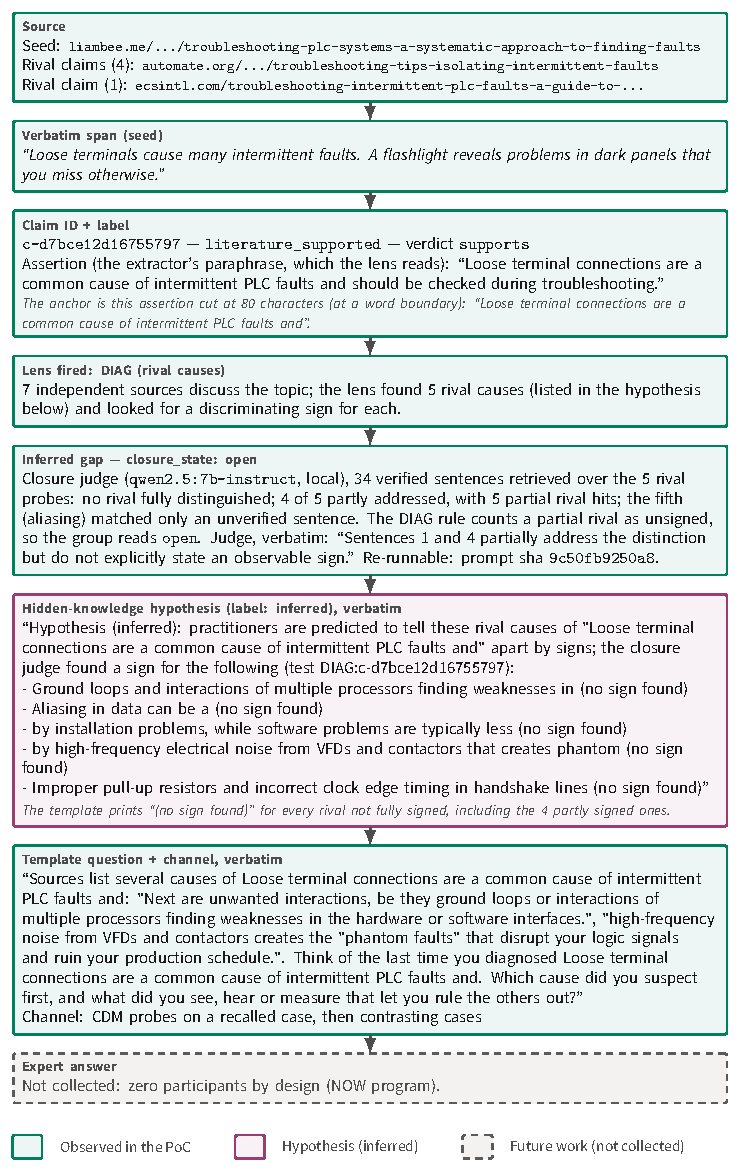
\includegraphics{figures/pdf/fig09_trace.pdf}
  \caption[One complete trace, source to question]{Trace 1, end to end: the seed span and its claim,
  the DIAG lens with five rival causes, the closure judge's verdict (no rival fully signed; 5 claims
  partly signed, which the DIAG rule counts as unsigned, so the record reads \code{open}), the
  hypothesis and the template question. The lens fired; the absence check found the element at most
  partly stated. No expert has answered the question.}
  \label{fig:trace}
\end{figure}

\textbf{Weaknesses.} The anchor is not a construct name but the extractor's assertion cut at 80
characters, so the question is not a grammatical sentence. The hypothesis template says the judge
\enquote{found a sign for the following} and then marks every item \enquote{(no sign found)}. The
\code{open} state overstates the evidence, since the judge found partial signs for several rivals.
The pre-review prototype showed a \emph{different} record on the same text (a DISC record on
\enquote{loose}); it is not in the final map.\footnote{\repo{docs/plans/n3-poc-lens-spec.md} \S9;
historical only.}

\subsection{Failure trace: a second fragment question}

PLC's second record shows the same template defect on a different anchor and a larger evidence
set.\footnote{\repo{research/n3/plc/gapmap.json}, \code{map[1]}, \code{gap_id}
\code{g-994077969379}.}

\begin{table}[tbp]
  \centering
  \small
  \caption{Failure trace: PLC, lens DIAG, gap \code{g-994077969379}, category HYP, closure
  \code{open}.}
  \label{tab:trace-fail}
  \begin{tabularx}{\linewidth}{@{}p{2.4cm}X@{}}
    \toprule
    Stage & Content \\
    \midrule
    Seed span and claim & \enquote{In a motion controller or PLC, it's often race conditions in
      user logic.} (\url{automate.org}); claim \code{c-ec36686ad589464b}, \code{literature_supported};
      assertion \enquote{Race conditions in user logic are a common source of intermittent faults in
      motion controllers and PLCs.} \\
    Lens \& target & DIAG: 11 independent sources discuss the topic; the lens found 7 rival causes,
      one of which is the fragment \enquote{array subscript out of range.} \\
    Inferred gap & Of 50 verified sentences retrieved, the judge found none that fully states a
      discriminating sign for any rival; it marked 6 claims as partial, so the group reads
      \code{open} by the DIAG rule \\
    Question \& channel & \enquote{[\ldots] Think of the last time you diagnosed Race conditions in
      user logic are a common source of intermittent faults in. Which cause did you suspect first,
      and what did you see, hear or measure that let you rule the others out?} (opening sentence
      with two quotes omitted) -- CDM probes on a recalled case, then contrasting cases \\
    \bottomrule
  \end{tabularx}
\end{table}

\textbf{Weaknesses.} The question is not a grammatical sentence, because the DIAG template splices
the anchor, the seed assertion cut at 80 characters, into a fixed frame. The rival causes are
fragments of the same kind (\enquote{Aliasing in data can be a}, \enquote{array subscript out of
range.}), and the judge's DIAG prompts are built from these same fragmentary cause strings. The
evidence is unaffected, but the closure judgment may be affected. A candidate that reads this poorly
should not reach an interview unedited.

\subsection{What these traces do, and do not, show}

\evobs{} The traces show that the mechanism runs end to end, from a real source span to a question
whose frame is fixed code, and where model-written text enters: the anchor, the rival causes and
some quotes come from the extractor's paraphrase (\cref{sec:n3}). \evint{} They cannot show, without
a human answer, whether any question would surface knowledge a practitioner holds. Both DIAG traces
are \code{open} only by the DIAG rule, and the closure step behind every record does not yet beat its
mismatched-evidence control (\cref{sec:absence-check}). These are candidates for a future interview, not findings.
